\chapter{Data analytics of public transport networks}


\section{Introduction and methods}
 The Citylines platform is a collaborative effort to map the public transport systems of the world \cite{Citylines}. It offers a dataset that contains a detailed history of the development of transport networks in several cities, from multiple countries. The aim of this task is to reconstruct the transport networks from the available data, and to perform an analysis of such networks. The first part of the task is concerned with the development of the methods and heuristics that are necessary to reconstruct and infer networks from the geographical location of nodes and edges. Each network is built as a set of connected components, where each connected component represents a public transport line, in which the nodes represent stations and edges are a simplified representation of the sections connecting the stations. The second part of the task is concerned with the analysis and characterisation of the produced networks, by means of standard topological descriptors.
 
 The construction of the transport network for a given city is done by iterating the same procedure for all available transport lines. First, all stations that are linked to the line are stored as nodes. Then, the edges between the nodes are built in a three--step process. Initially, each node attempts to connect to its two closest neighbours, using their geographical location as position. The connection is accepted unless the neighbours are closer to each other than to the reference node, in which case the edge is only added between the reference node and its closest neighbour. Then, for every section of the line, an edge between the two nodes that are closest to the respective ends is attempted. In this case, the edge is rejected if there already exists a path between the nodes. Finally, a rewiring step is performed to avoid spurious edges: for each two connected nodes, if a shorter edge between one of the nodes and a neighbour is possible then the original edge is replaced by the shorter alternative. This rewiring is repeated until no more replacements are possible. A check is performed throughout the entire process so that the same edge is not built multiple times.
 
The analysis and characterisation of the transport networks is done by means of topological descriptors. To take into account any possible relationship between topology and size, the networks are classified into small ($N < 100$), medium ($100 \leq N < 500$) and large ($N \geq 500$) according to the amount of nodes $N$. Additional details on the methodology can be found in section \ref{sec:DATN_SM} of the Supplementary Material.


\section{Results and discussion}

Fig. \ref{fig:degree_dist_cities} presents the degree distribution of small, medium and large cities. It can be noted that the distribution does not change significantly between different city sizes. The large ratio between $P(k=2)$ and $P(k=1)$ may indicate that transport networks consist of few lines composed of many stations. In particular, this appears to be less notable for small cities. Additionally, the low proportion of nodes with $k=3, 4$ points towards transport lines having a low amount of branches.

The average shortest path length, $I_G$, is shown in Fig. \ref{fig:avg_path_length_cities} as a function of the number of nodes $N$, both for the largest connected component (LCC) and as an average over all connected components. For the LCC, the shortest path appears to scale as $I_G\propto \log(N)$, while for the average over all connected components it seems to scale as $I_G\propto \sqrt{\log(N)}$. 

\begin{figure}[!h]
	\begin{center}
	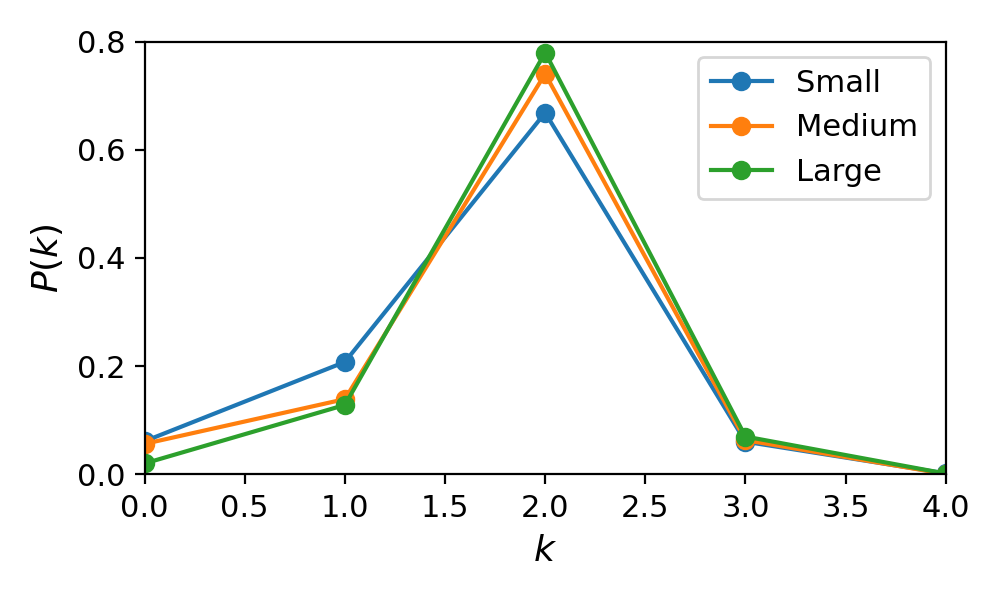
\includegraphics[scale=0.75]{./images/task_41/degree_dist_cities.png} 
	\end{center}
	\caption{Degree distribution, $P(k)$, for city transport networks. Results are shown for small, medium and large cities.\\} 
	\label{fig:degree_dist_cities} 
\end{figure}


\begin{figure}[!h]
	\begin{center}
	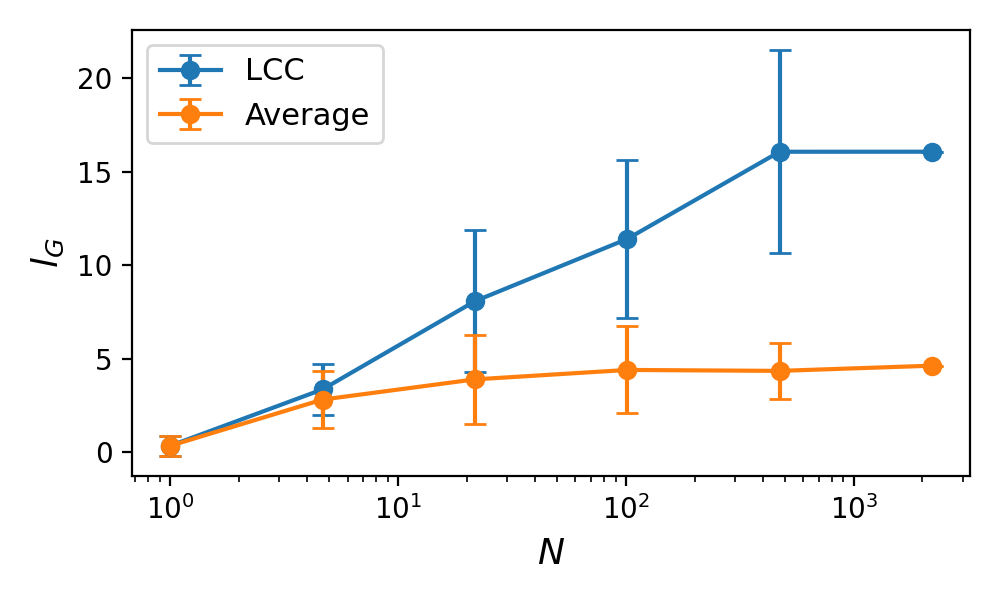
\includegraphics[scale=0.75]{./images/task_41/avg_path_length_cities.png} 
	\end{center}
	\caption{Average shortest path length, $I_G$, with respect to the number of nodes, $N$, for city transport networks. The results are presented for the largest connected component of the network (LCC), as well as for the average over all connected components. \\} 
	\label{fig:avg_path_length_cities} 
\end{figure}


\newpage